
\section{Optimización univariada}


    \begin{definicion} Sea $f:D\subset \R \to \R.$ Decimos que:
        \begin{enumerate}
            \item $f$ alcanza su \emph{valor máximo} o \emph{máximo global} en $c\in D$ si $f(c)\geq f(x),$ para toda $x\in D$;
            \item $f$ alcanza su \emph{valor mínimo} o \emph{mínimo global} en $c\in D$ si $f(c)\leq f(x),$ para toda $x\in D$.
        \end{enumerate}
        
    \end{definicion}


    \begin{teorema}[Teorema del Valor Extremo]
        Si $f:[a,b]\to \R$ es continua, entonces $f$ alcanza su máximo y su mínimo.
    \end{teorema}


    Aunque el criterio anterior nos es útil al optimizar en intervalos compactos, es decir, de la forma $[a,b]$, en un caso
    general no siempre esto es cierto. Sin embargo, tenemos la siguiente noción de máximo (mínimo) en intervalos abiertos.


    \begin{definicion} Sea $f:D\subset \R \to \R.$ Decimos que:
        \begin{enumerate}
            \item $f$ tiene un \emph{máximo local} en $c\in D$ si existe un radio $\ep>0$ suficientemente pequeño, de
            manera que $f(c)\geq f(x),$ para toda $x\in (c-\ep,c+\ep)\subset D$;
            \item $f$ tiene un \emph{mínimo local} en $c\in D$ si existe un radio $\ep>0$ suficientemente pequeño, de
            manera que $f(c)\leq f(x),$ para toda $x\in (c-\ep,c+\ep)\subset D$.
        \end{enumerate}
        
    \end{definicion}


    \begin{observacion}
        La condición de que exista si existe un radio $\ep>0$ suficientemente pequeño, y que $x\in (c-\ep,c+\ep)\subset D$ se
        puede entender como que $x\in D$ este suficientemente cerca de $c\in D.$ De manera informal, podemos decir que $f$
        alcanza un máximo local en $c$ si $f(c)\geq f(x)$ para $x$ suficientemente cercanos a $c.$ Lo mismo se puede decir para
        un mínimo local. Note que todo máximo (mínimo) global es, en particular, un máximo (mínimo resp.) local.
    \end{observacion}


    \begin{teorema}[Teorema de Fermat]
        Si $f:D\subset \R \to \R$ alcanza un máximo o mínimo local en $c\in D$ y $f'(c)$ existe, entonces \emph{necesariamente}
        $f'(c)=0.$
    \end{teorema}


    \begin{observacion}
        Debemos tener cuidado al usar el teorema de Fermat. Por ejemplo $f=\abs{x}$ alcanza su mínimo en cero, pero en este
        punto la derivada no existe. En cambio, $f(x)=x^{3}$ tiene derivada igual a cero en $x=0,$ pero este punto no es máximo
        ni mínimo de la función.
    \end{observacion}


    Como podemos apreciar, los puntos más interesantes para nuestro estudio son aquellos donde la derivada no existe o si
    existe, es igual a cero.


    \begin{definicion}
        Sea $f:D \subset \R \to \R$ y $c\in D.$ Decimos que $c$ es un punto crítico si $f'(c)$ no existe o si existe,
        $f'(c)=0.$
    \end{definicion}


    Con los resultados anteriores, podemos describir un criterio para optimizar funciones continuas en compactos.


    \begin{proposicion}
        \label{opt:compacto}
        Supongamos que
        \begin{enumerate}
            \item $f:[a,b]\to \R$ es continua,
            \item $f:(a,b)\to \R$ es diferenciable.
        \end{enumerate}
        Si $f$ alcanza su máximo (o mínimo) global en $c,$ entonces
        \begin{enumerate}
            \item $c=a$ o $c=b,$ o
            \item $f'(c)=0$ un punto crítico.
        \end{enumerate}
    \end{proposicion}


    En decir, para encontrar donde $f$ alcanza sus valores extremos, basta probar en los extremos del intervalo o en los
    puntos críticos, que se encuentran en su interior.


    \begin{problema}
        Encuentre el máximo y el mínimo global de la función $f(x)=x^{3}-3x^{2}+1$ si $-\frac{1}{2}\leq x \leq 4.$
    \end{problema}

{Solución}
    
    \begin{figure}
        \centering
        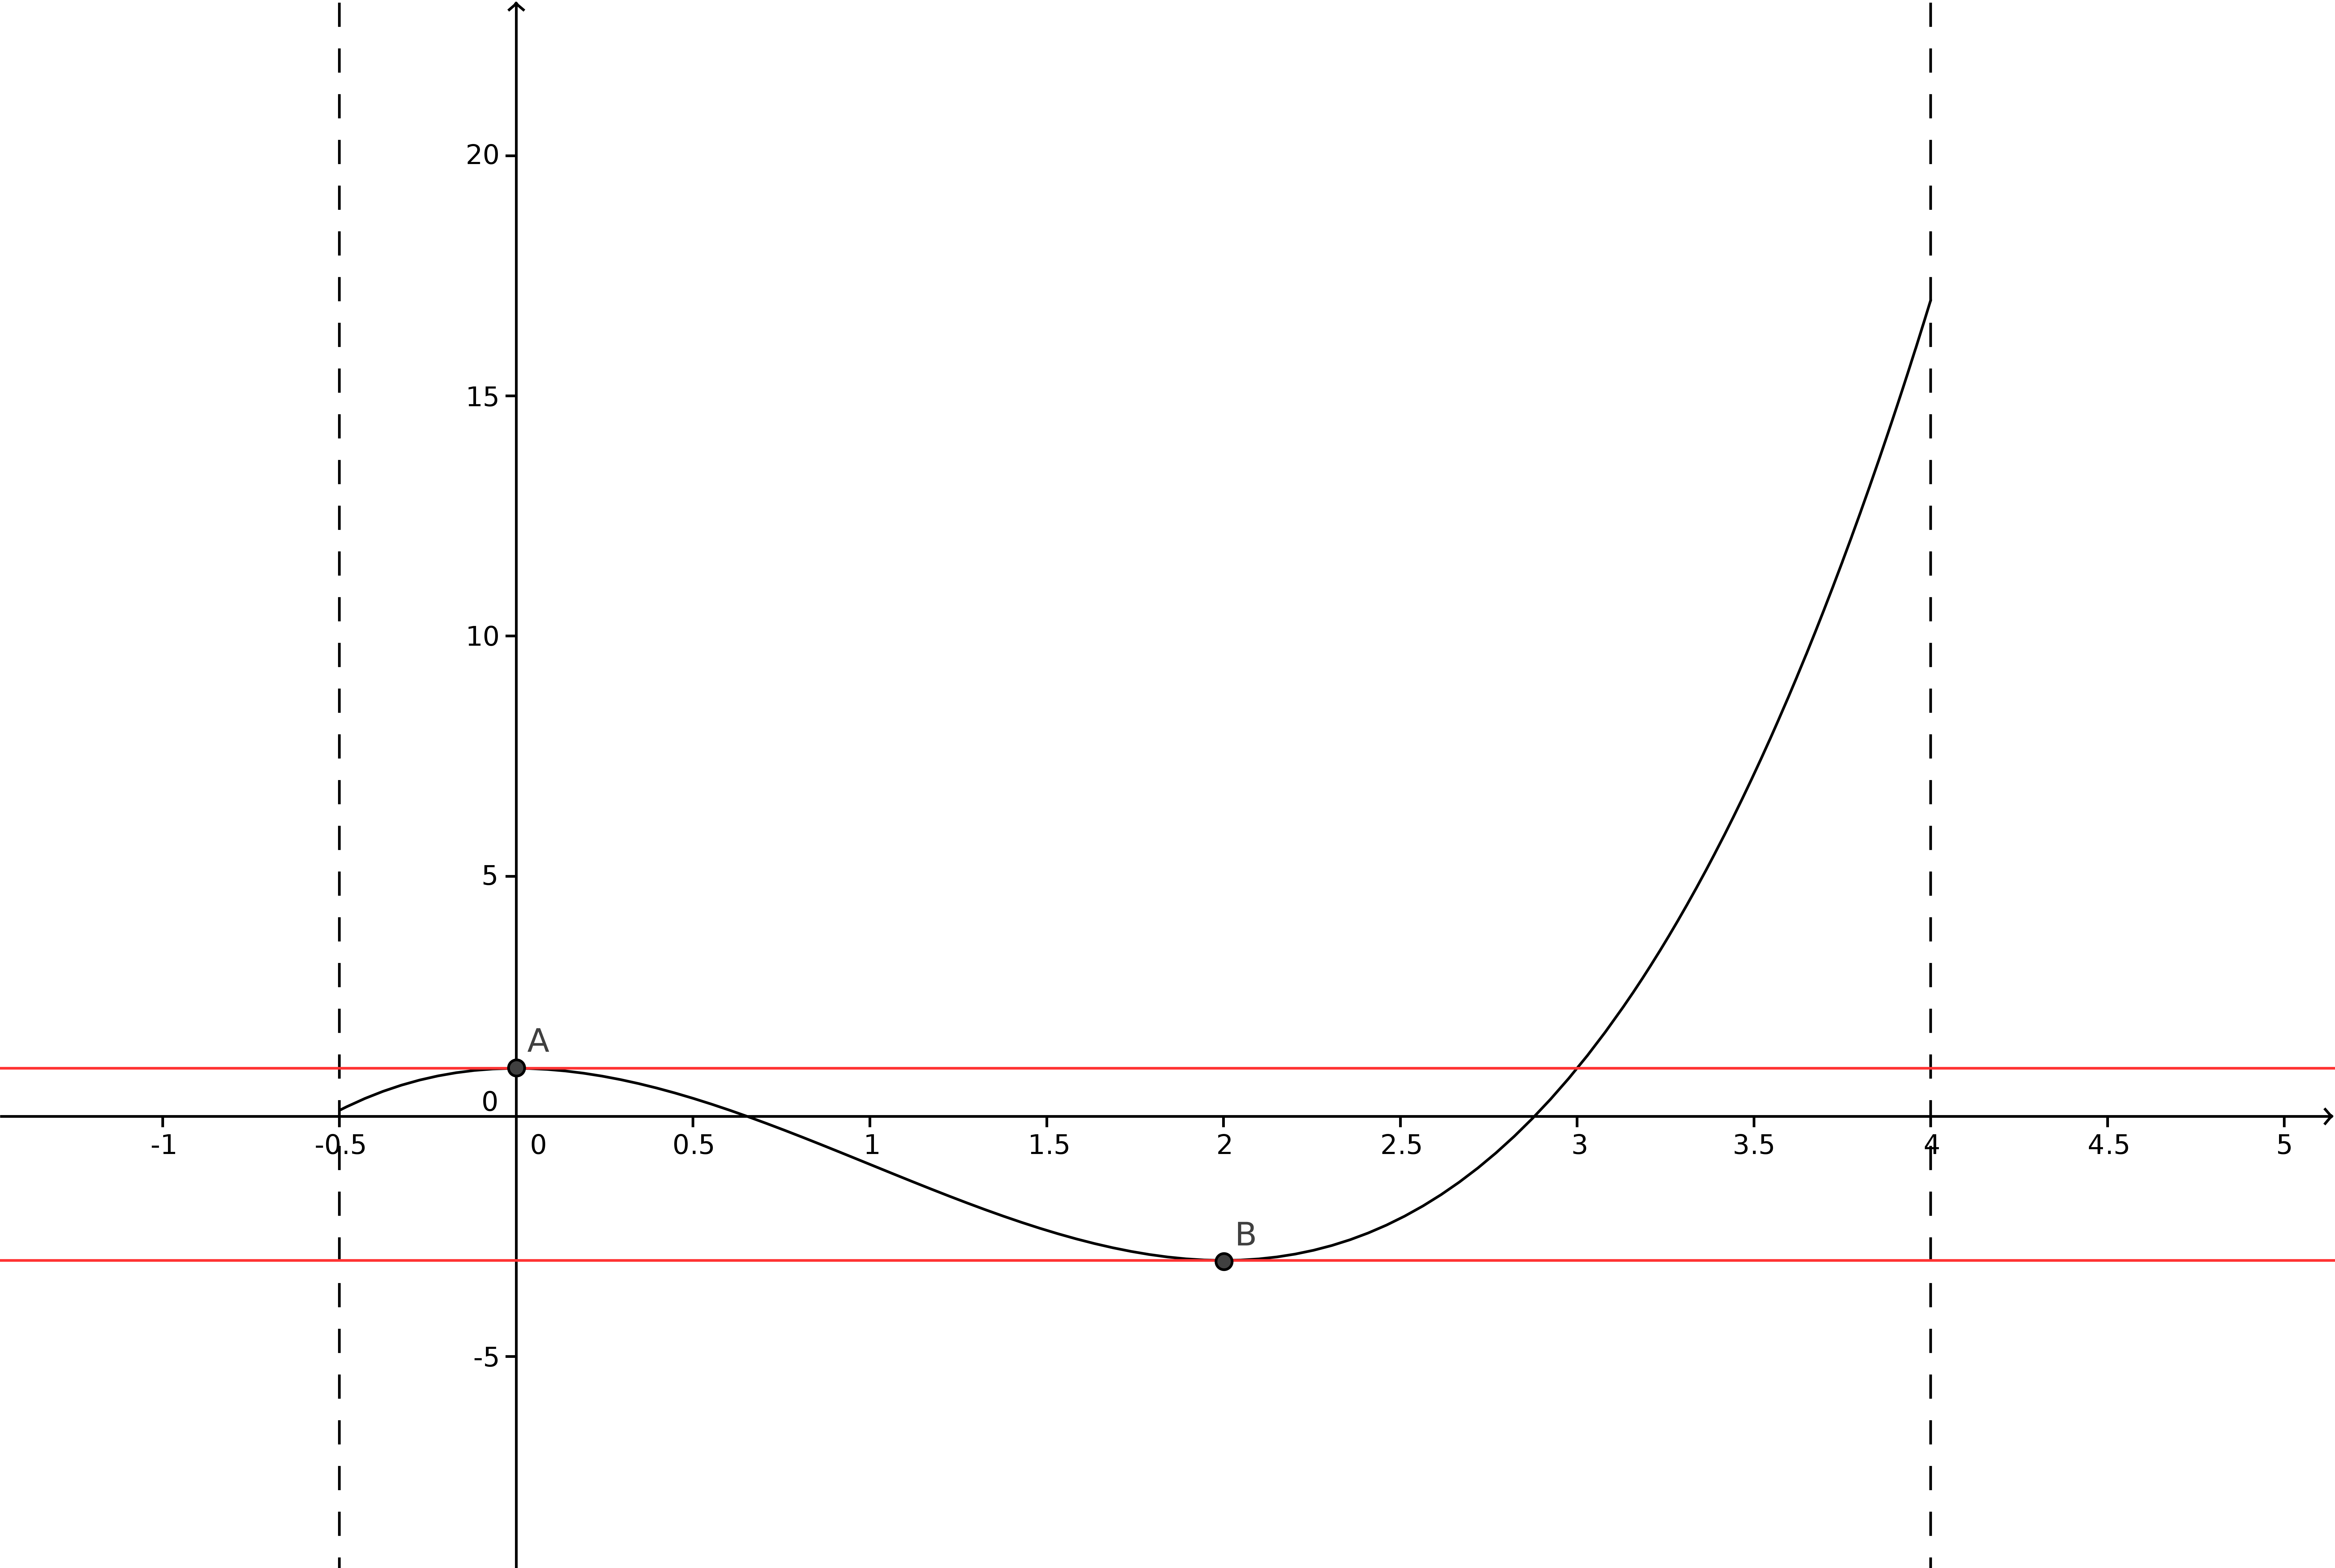
\includegraphics[height=3cm,keepaspectratio=true]{./calculo/optimizacion.png}
        % optimizacion.png: 7799x5238 pixel, 300dpi, 66.03x44.35 cm, bb=0 0 1872 1257
        \caption{$f(x)=x^3-3x^2+1$}
        \label{fig:optimizacion}
    \end{figure}



    Como $f$ es continua en $[-\frac{1}{2},4]$ y diferenciable en su interior $(-\frac{1}{2},4)$ (¿porqué?), podemos
    aplicar el criterio de la proposición \ref{opt:compacto}.
    
    
    
    Primero evaluamos en los extremos.
    $$
    \begin{cases}
        f(-\frac{1}{2})=\frac{1}{8} \\
        f(4)=17
    \end{cases}
    $$
    
    Derivamos $f$ y obtenemos los puntos críticos, resolviendo la ecuación
    $$
    f'(x)=3x^{2}-6x=3x(x-2)=0.
    $$
    
    Los puntos críticos son $x=0$ y $x=2.$ Sus respectivos valores son $f(0)=1$ y $f(2)=-3.$
    
    Finalmente, basta comparar los diferente valores obtenidos para concluir que el máximo global es $17$ y se alcanza en
    $x=4$, mientras que el mínimo global es $-3$ y se alcanza en $x=2.$
    
    


    
    \begin{problema}
        Encuentre los máximos y mínimos absolutos en el intervalo indicado. Grafique.
        \begin{enumerate}
            \item $f(x)=2x^{3}-3x^{2}-12x+1, \, [-2,3]$
            \item $f(x)=\frac{x}{x^{2}-x+1}, \, [0,3]$
            \item $f(x)=t\sqrt{4-t^{2}}, \, [-1,2]$
            \item $\phi(t)=2\cos(t)+\sin(2t), \, [0, \frac{\pi}{2}]$
            \item $f(x)=xe^{-x^{2}/8}, \, [-1,4]$
            \item $f(x)=\ln(x^{2}+x+1), \, [-1,1]$
            \item $f(x)=x-2\arctan(x), \, [0,4]$
        \end{enumerate}
        
    \end{problema}


\subsection{Optimización aplicada}


	\begin{problema}
		Una caja abierta está hecha al cortar pequeños cuadrados congruentes, de las esquinas, de una hoja de lata de \texttt{12 in} por \texttt{12 in}, y doblando los lados hacía arriba. 
		
		¿Qué tan largas deben ser las esquinas cortadas de las esquinas para hacer la caja tan grande como sea posible?
	\end{problema}



	\begin{figure}
		\centering
		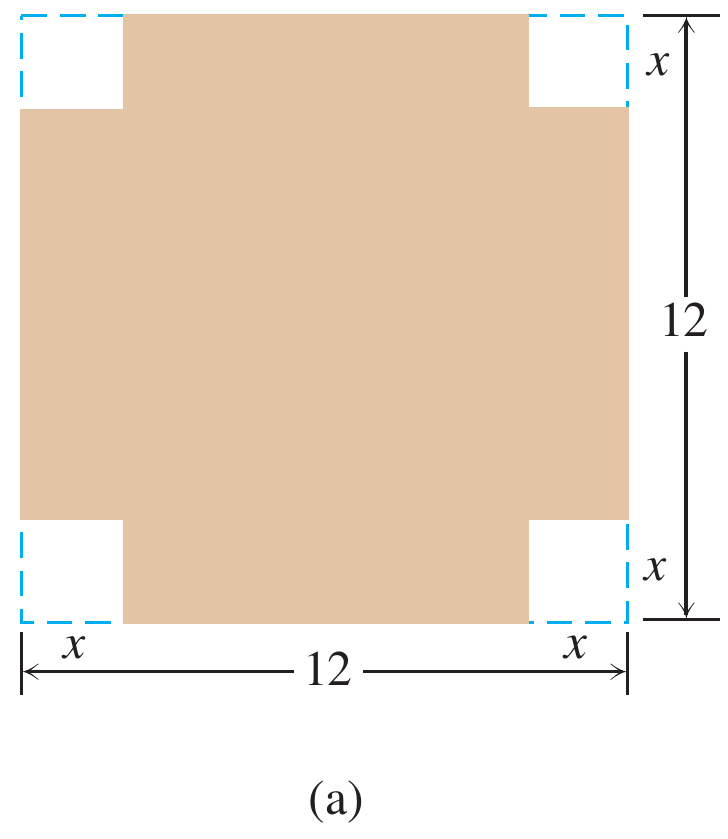
\includegraphics[height=0.7\textheight]{./calculo/thomas_04_36_a}
		\label{fig:thomas0436a}
	\end{figure}
	



	\begin{figure}
		\centering
		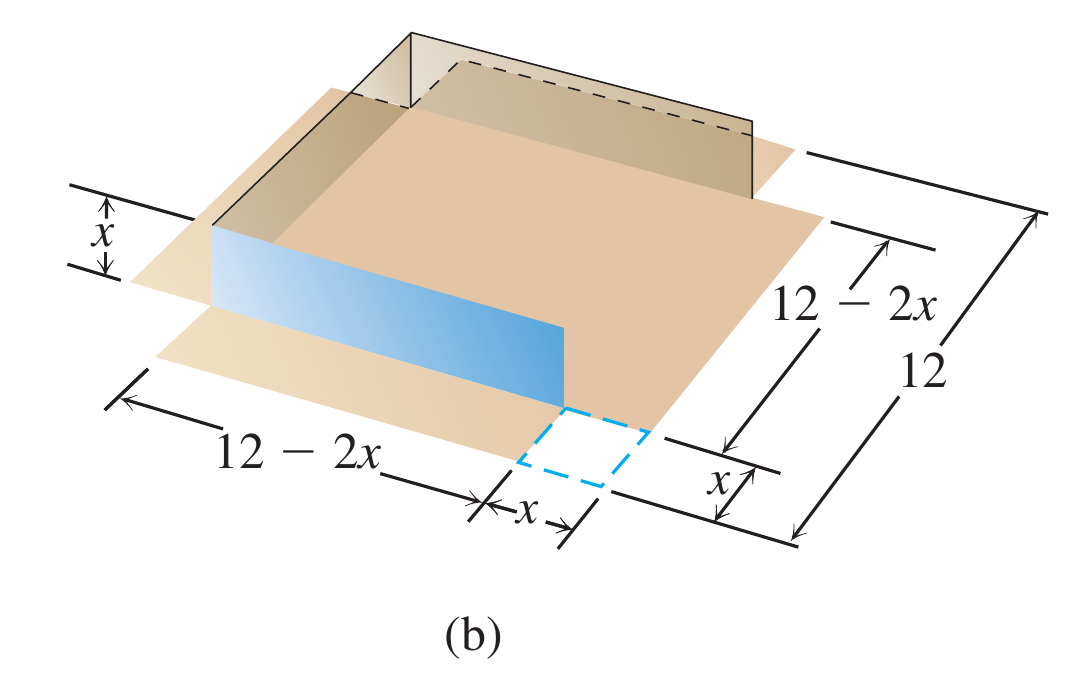
\includegraphics[width=0.7\textwidth]{./calculo/thomas_04_36_b}
		\label{fig:thomas0436b}
	\end{figure}
	



	
	Se te ha pedido diseñar una lata de un litro, con la forma de un cilindro circular recto. ¿Qué dimensiones utilizarán el menor material posible?



	
	\begin{figure}
		\centering
		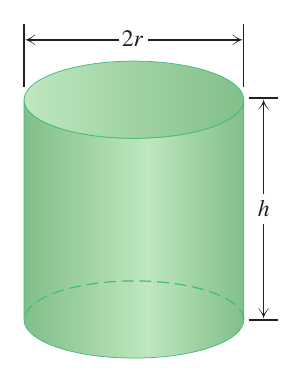
\includegraphics[height=0.7\textheight]{./calculo/thomas_04_38}
		\label{fig:thomas0438}
	\end{figure}
	



	Un rectángulo está inscrito en un semicírculo de radio 2. ¿Cuál es el área más grande que se puede obtener, y cuáles son las dimensiones?
	



	\begin{figure}
		\centering
		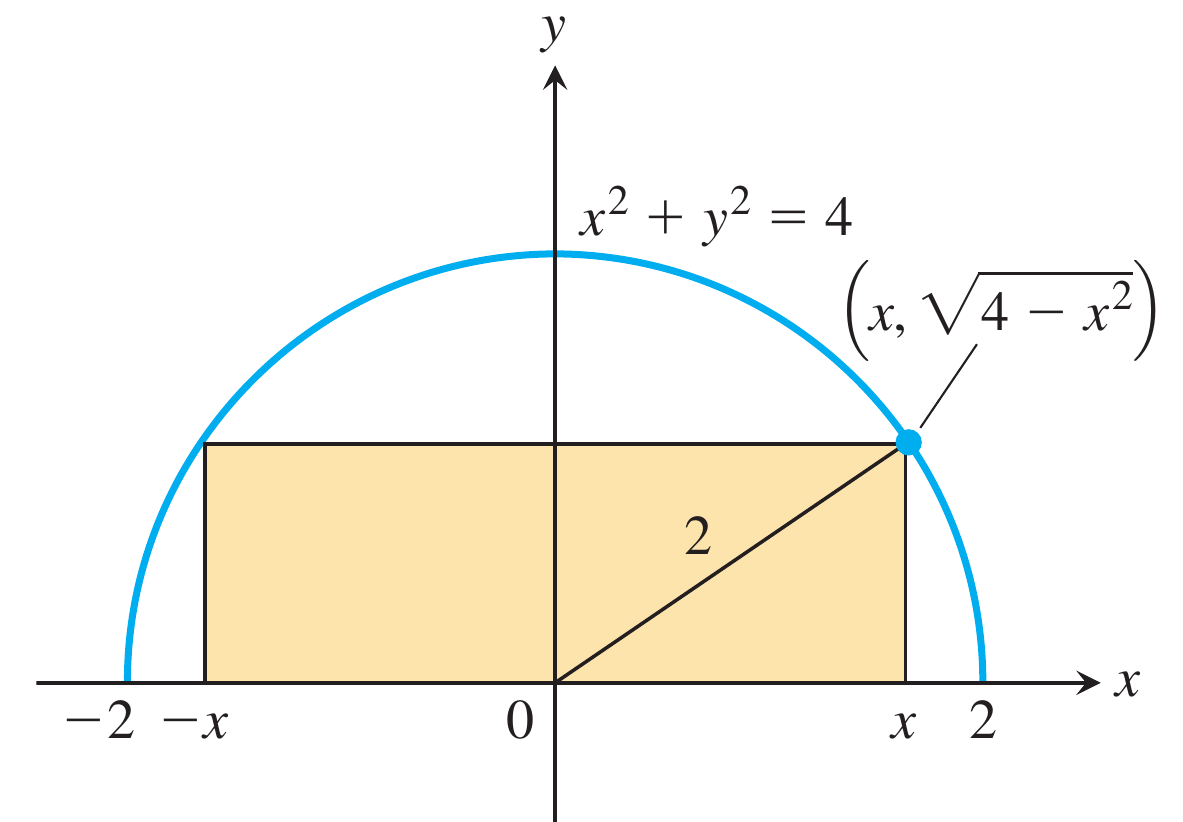
\includegraphics[height=.7\textheight]{./calculo/thomas_04_40}
		\caption{}
		\label{fig:thomas0440}
	\end{figure}
	


[Ley de Snell (refracción)]
	La velocidad de la luz depende del medio a través del cuál viaje, y es generalmente más lenta en medios más densos. 
	
	 
	
	El \emph{principio de Fermat} (de óptica) establece que la luz viaja fe un punto a otro a lo largo de un camino para el cual el tiempo es mínimo. 
	



		\begin{figure}
		\centering
		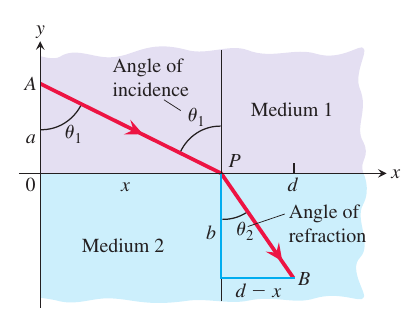
\includegraphics[height=.7\textheight]{./calculo/thomas_04_41}
		\caption{}
		\label{fig:thomas0441}
	\end{figure}
	Describe el camino para el cuál un rayo de luz seguirá yendo de un punto $A$ en un medio en el que la velocidad es $c_1$, a un punto $B$ en un medio en el que la velocidad es $c_2$.


